%----------------------------------------------------------------------------------------
%----------------------------------------------------------------------------------------
%----------------------------------------------------------------------------------------
%Method
%----------------------------------------------------------------------------------------
%----------------------------------------------------------------------------------------
%----------------------------------------------------------------------------------------

\section{METHOD}
\label{sec: method}
 \subsection{Self Organizing Maps}
 \label{sec: som}
 
 The self-organizing map is a clustering method which reduces the dimension of the data, usually to one or two dimensions (1D or 2D), while preserving topological features of the original dataset.
 The result of an SOM is a set of nodes (neurons) that are arranged in a 1D or 2D arrays \citep{Kohonen98}. 
 Each node may contain one or more samples from the input data.
 The distance between the nodes represents similarity or dissimilarity of the underlying samples, i.e., similar data are closer together in the array and the distance between two nodes is related to the dissimilarity of their samples.
 A weight vector ``\boldit{W}" with the same dimension as the input data is associated with each node and will be varied during the training process.
 This vector is the key factor in determining the position of the nodes in a map.
 \cite{Geach12} presented the application of the SOM and discussed its algorithm in detail.
 In this section we briefly discuss the algorithm of SOM, how we create our maps and a present a mock model which will help interpretation of our results. %%%Sr220616: changed a test model to a mock model
 
 \subsubsection{Algorithm of SOM} 
 \label{sec: algorithm}
     Assume we have a dataset which contains vectors, \boldit{V} $\in \Re^n$, and we want to map them on an S1 by S2 map.  %%%Sr220616: moved paraghraph regarding to the size here!
     The sizes of the SOM maps are arbitrary and there are no rules regarding choosing one over the other. 
    \citet{Vesanto05} suggested that a total number of $5\sqrt{n}$ neurons is a sufficient size, but users usually choose the size of the grids based on their dataset and their application of the results.

     We start by creating S1 $\times$ S2 empty neurons. 
     The arrangement of these neurons depends on the map's topology provided by the user. %%%Sr220616: removed initial from here, it is fixed after choosing the topology.
     In the case of 1D maps, since each neuron has two immediate neighbours, the topology of the map does not have any effect on the final result and any topology can be chosen.
     However, in 2D maps, the shape of the neurons specifies the number of immediate neighbours for each neuron and it is up to user to choose the most suitable shape based on the data.
     In this paper, we choose hexagonal topology, which gives each neuron six neighbours, and provides more interactions between neurons.
     Initially a random weight vector, \boldit{W} $\in \Re^n$, will be assigned to each node.
     The process of creating SOM happens over a series of $N$ iterations, which is set by a user. %%% SR220616: added here that N is set by a user
     During each iteration the weight vectors might change according to the Kohonen learning rule (equation~\ref{equ: weight adj}). 
      In each iteration, the SOM code:
     \begin{enumerate}
        \item chooses a random vector from the dataset ($V_i$).
        \item calculates the Euclidean distance in $\in \Re^n$ space for each node, $j$, as  $D_j^2= \sum_{i=0}^{i=n} (V_i - W_i)^2$, and finds a neuron with minimum $D_j$, (``$D_{j_{min}}$"). This neuron is the winner node and is called the Best Matching Unit (BMU). %%%Sr220616: added $\in \Re^n$ space to be more clear on that it is a distance in n-dimension space no neurons!
        \item  computes the radius of the neighbourhood of the BMU to find nodes within this radius. The weight vectors of these nodes will be affected in the next steps. The radius of the neighbourhood is arbitrary and can be set to be as high as half of the SOM size. It then decays exponentially over each iteration as
        \begin{equation}
            r^t_{BMU} = r^0_{BMU}e^{(-t/\tau)}
        \end{equation}
        where $\tau$ is a decay constant and is usually set to be the same as the number of iterations, $N$. $r^0_{BMU}$ and $r^t_{BMU}$ are the radii of the neighbourhood at 0th and $t$th iteration, respectively. 
        \item changes the weight vectors of the BMU and all the nodes within $r^t_{BMU}$ as:
        \begin{equation}
            \label{equ: weight adj}
            w(t+1)=w(t)+L(t) \times R(t) \times(v(t)-w(t))
        \end{equation}
        where $L(t) = L_0 e^{(-t/\tau)}$ is the learning factor, which prevents the divergence of the SOM and $R(t)=\exp(-\frac{D_j^2}{2r^t_{BMU}})$ is the influence rate. $R(t)$ determines how the weight of each node in the neighbourhood of BMU will change.
     \end{enumerate}
     These steps are then repeated $N$ times.
     
\subsection{Creating self-organizing maps}
\label{sec: create_som}
     In order to create SOMs, we use {\sc matlab} neural network toolbox~\citep[NNT,][]{matlabtolbox}.
     SOM in {\sc nnt} can be created by {\sc newsom} or {\sc selforgmap} library, both of which work in two phases, an ``ordering phase" and a ``tuning phase". 
     The first phase is called the ``ordering phase" and
     starts with maximum neighbourhood distance and an initial high learning factor (usually 0.9) is provided by the user. 
     The ordering phase continues for a requested number of iterations.
     During the iterations, the learning factor decreases to the tuning phase learning factor and the neighbourhood distance reaches that of the tuning phase as well.
     Both the learning factor and the neighbourhood of the tuning phase are set by the user. 
     The amount by which these two factors change in each iteration depends on the number of iterations.
     
     In the second, or ``tuning'' phase,
     the neighbourhood distance is kept at the user-defined minimum.
     The learning factor, however, decreases gradually.
     The gradual change in the leaning factor helps to fine-tune the topology results, leading to a more stable SOM. 
     To allow the fine tuning, the number of iterations in this phase must be much larger than the that of the ordering phase. %cite kohenen book?!
     We chose the number of epochs in the tuning phase to be 3 times the number of epochs in the ordering phase.
     
     We create the final SOMs with initial values for number of iterations in ordering phase, ordering phase learning factor, tuning phase learning factor, and tuning phase neighbourhood distance of 1000, 0.9, 0.02, and 1, respectively. %%%Sr220616: moved this sentence from the result part to here!
     To present our results, we use {\sc nnt}'s built-in plotting tool.
%     This tool is designed to show the distance between each cluster more clearly.
     Specifically, we use two of the plots in this tool: a hits map, which shows the number of times each neuron has became the winner (hits), and a distance map, which shows the distance between those neurons.
     In the maps, the purple hexagonal shapes represent the neurons. 
     The distances in a distance map are shown by the grey cycle colours:
     the darker the colour, the larger the distance between neurons.
     In the hit maps, neurons with zero hits are left empty.
      
    
   
\subsection{Mock sample}
 
         \begin{figure}
            \begin{subfigure}[b]{0.5\textwidth}
                \centering
                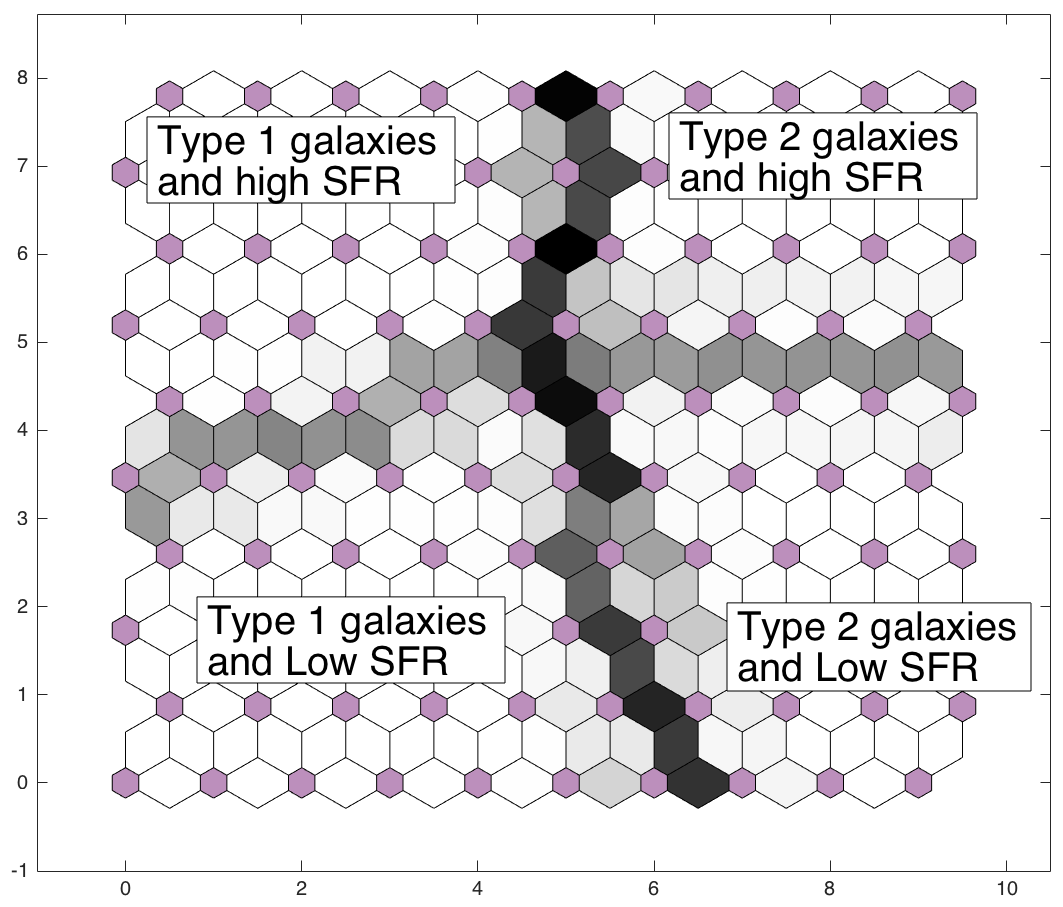
\includegraphics[width=\textwidth]{images0.01/sample/sample2_dist.png}
            \end{subfigure}
            \hfill
            \begin{subfigure}[b]{0.5\textwidth}
                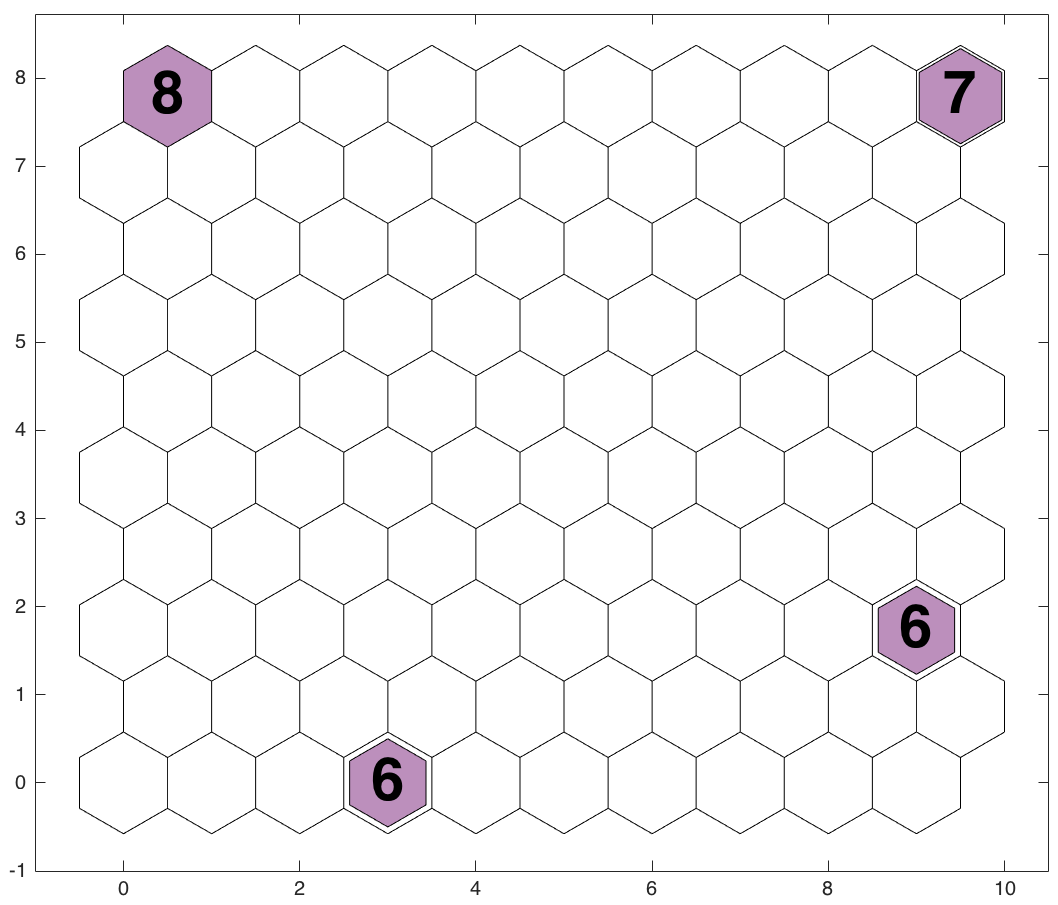
\includegraphics[width=\textwidth]{images0.01/sample/sample2_hits.png}
            \end{subfigure}
            \caption{SOM of the mock sample. In both plots, the axes show the position of the neurons. Hexagonal shapes represent the neurons. The top plot is a distance map. The grey cycle colours show the differences between the weights of each neuron with white being the minimum difference and black being the maximum one. The lower plot is a ``hits plot". It represents the number of samples in each neuron, where empty means zero hits. In this sample, the 27 galaxies are clustered in 4 groups, containing 8, 7, 6 and 6 galaxies respectively.}
            \label{fig: sample}
        \end{figure}
 
 To illustrate how self-organizing maps work, we create a mock sample of 27 galaxies.
 The mock sample contains two assigned attributes for each galaxy: the type (type 1 or type 2), and the star formation rate (high or low). 
 We generated a SOM of size $10 \times 10$ using the same initial values mentioned in Section ~\ref{sec: create_som}.

 Fig. ~\ref{fig: sample} shows the SOM of this mock sample. 
 The upper panel is the distance map. 
 The axes show the position of the neurons in the $10 \times 10$ network.
 The lower panel in Fig.~\ref{fig: sample} shows the hit map.
 On this map, similar to the distance map, the axes show the position of the neurons and the hexagonal shapes are the neurons.
 The number on the purple neurons shows the number of galaxies in that neuron.
 Colour coverage of neurons depends on the number of the hits on the sample.
 The neuron with the maximum number of hits is fully coloured while the empty neurons are left uncoloured (white). %%%Sr220616:changed the dark-coloured to fully coloured
 
 
Using this method, as expected, we are able to divide the mock sample galaxies into 4 distinct groups: Type 1 with high SFR, type 1 with low SFR, type 2 with high SFR and type 2 with low SFR. 
The upper panel in the Fig.~\ref{fig: sample} clearly shows this division.
In that plot, the upper half belongs to high star forming galaxies, while the lower half belongs to low star forming galaxies.
The left half of the plot is where type 1 galaxies belong, and type 2 galaxies reside in the right side.
Different shades of gray show the border between regions.
The lower panel in Fig.~\ref{fig: sample} shows that only 4 neurons (out of 100) are occupied. 
8 galaxies are type 1 galaxies with high SFR, 7 are type 2 galaxies with high SFR, 6 are type 1 galaxies with low SFR and the other 6 are type 2 galaxies with low SFR. 

%%%Sr220616:added a paragraph here
We can conclude that although each galaxy had the chance to occupy any of the neurons in the network, because of the similarity in the values of their attributes, they remained only in four groups.
This network is considered a training network and can be used to cluster any new dataset with similar entries.
Some neurons were left empty in this network because they never had became a winner for data in the mock sample.
However, their weights have been updated in each iteration, and they could be a winner for data in the new dataset.%%%Sr220616: added the last two sentences to clear out a confusion about empty neurons.

As we show in the following sections, with data from real galaxies there are more than two dimensions and two galaxies never have exactly the same information. 
If the network has enough neurons, the input data points would eventually separate from each other and cluster into smaller groups. 
However, if the input data has high similarity, the number of neurons must be much higher than the number of input samples to be able to separate the groups from each other. 
Therefore, it is up to the users to decide the similarity or dissimilarity between the input data based on number of neurons. 
